\pagenumbering{arabic}
\setcounter{page}{10}
\section{Introducción}

	Una de las necesidades principales del ser humano es la de la comunicación, éste tiene la necesidad de ser escuchado y de interactuar con los demás seres vivos en especial con otros humanos, la comunicación nos ayuda a compartir sentimientos, es una forma de expresarnos \cite{VelezMelendez2004}.

	En la vida diaria tenemos diversas formas de comunicarnos, puede ser con señales acústicas (voz, sonidos, ruidos), visualmente, por medio de medios impresos, la escritura, dibujos, señas, etc. El objetivo es mandar un mensaje, básicamente se puede describir la comunicación mediante el diagrama de la Figura \ref{comunicacion}.

	\begin{figure}[H]
		\centering
		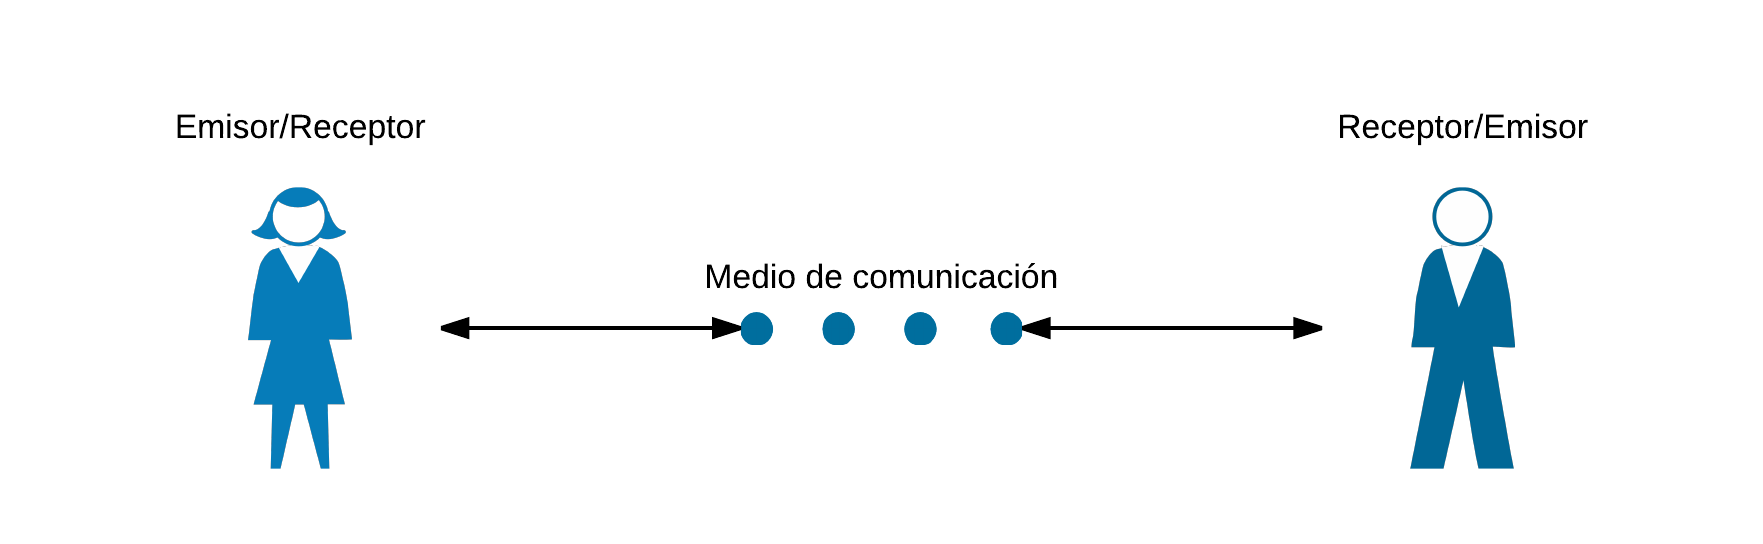
\includegraphics[scale = 1]{figures/Comunicacion}
		\caption{Elementos de comunicación.}
		\label{comunicacion}
	\end{figure}

	La comunicación oral nos ofrece grandes ventajas sobre los demás métodos de comunicación pues es el modo de comunicación más natural entre nosotros los humanos, la gran ventaja es que no es necesario estudiarla, es parte de nuestro crecimiento, aprendemos a hablar, adoptamos el idioma, el acento, las costumbres, en cambio el modo de comunicación escrita requiere de un estudio del alfabeto, escritura y lectura, además de que la comunicación oral nos permite inducir más significados a las palabras que su propia definición gracias al tono de voz \cite{CamargoLopez}.

	Pero no todos tenemos la capacidad de comunicarnos de forma oral, hay personas que no pueden hablar u oír ya sea porque nacieron con esta deficiencia o porque por alguna razón físicamente se vieron limitados a realizar tal actividad.

	La discapacidad es una condición que puede afectar a cualquier miembro de la sociedad sin importar edad, sexo, estatus social-educativo-laboral o educación geográfica \cite{Flores}. Como consecuencia se tienen deficiencias en el rendimiento de la actividad cotidiana de la persona como en la ejecución de tareas, actitudes y conductas \cite{Flores}.

	Desarrollar una aplicación móvil que pueda eliminar esta barrera de comunicación puede ser una herramienta muy útil para que las personas con discapacidad auditiva no pierdan la comunicación o aprendan a comunicarse con el resto de las personas y de esta forma la interacción no esté limitada en ambos sentidos.